% =====================================================================================
%  HW2 — Informe tecnico
%  Todas las tablas y figuras se generan desde el pipeline (`python run_pipeline.py`).
%  Ninguna cifra de este documento esta tecleada a mano: las tablas se leen con \input
%  desde report/tablas/ y las figuras desde report/figures/.
%  Compilar con:  python run_pipeline.py --phase 5
% =====================================================================================
\documentclass[11pt,a4paper]{article}

\usepackage[T1]{fontenc}
\usepackage{lmodern}
\usepackage[spanish,es-nodecimaldot]{babel}
\usepackage[margin=2.5cm]{geometry}
\usepackage{booktabs}
\usepackage{graphicx}
\usepackage{float}
\usepackage{caption}
\usepackage{xcolor}
\usepackage{hyperref}
\usepackage{siunitx}

\hypersetup{colorlinks=true, linkcolor=black, citecolor=black, urlcolor=blue!60!black}
\captionsetup{font=small, labelfont=bf}
\graphicspath{{figures/}}
\setlength{\parskip}{0.4em}
\setlength{\parindent}{0pt}

\title{\textbf{La hora dorada}\\[0.3em]
\large Accesibilidad por carretera a establecimientos de salud con capacidad
resolutiva en Lambayeque, Ayacucho y Loreto}
\author{José Miguel Díaz}
\date{Corte de datos: 31 de agosto de 2026 \\ \small Documento generado automáticamente
por el pipeline del repositorio}

\begin{document}
\maketitle

% =====================================================================================
\begin{abstract}
\noindent
Se mide el tiempo de viaje por red vial real desde \num{15418} centros poblados hasta el
establecimiento de salud con capacidad resolutiva más cercano, en tres departamentos
peruanos elegidos uno por región natural. El \SI{72.2}{\percent} de los
\num{2732389} habitantes del ámbito alcanza uno en menos de una hora, pero el
\SI{12.2}{\percent} \textbf{no lo alcanza por carretera en absoluto}. El contraste
geográfico domina el resultado: la población sin acceso vial es del
\SI{0.8}{\percent} en Lambayeque, \SI{4.3}{\percent} en Ayacucho y
\SI{38}{\percent} en Loreto. En la Amazonía el centro poblado mediano está a
\SI{8.9}{\kilo\meter} de la carretera más próxima, frente a \SI{107}{\meter} en la costa,
y su población rural tarda de media \num{23} horas. Solo \num{48} de los \num{2838}
establecimientos del ámbito son resolutivos. El problema no es de cantidad sino de
concentración geográfica: medir el acceso amazónico con una red vial es, en buena medida,
la pregunta equivocada.
\end{abstract}

% =====================================================================================
\section{Introducción y planteamiento del problema}

En el Perú los puestos de salud de categoría I-1 pueden estabilizar a un paciente, pero no
operar ni practicar una cesárea. Solo los establecimientos de categoría \textbf{II-1 en
adelante} disponen de capacidad resolutiva. En una emergencia obstétrica o un trauma grave,
esa distinción decide el desenlace: es lo que la medicina de urgencias llama la
\emph{hora dorada}.

La pregunta que guía este trabajo es:

\begin{quote}
¿Cuánto tarda \emph{realmente}, por carretera, la población de una región en llegar a un
establecimiento de salud con capacidad resolutiva, y dónde están las peores brechas?
\end{quote}

La palabra \emph{realmente} impone dos exigencias. La primera es metodológica: la distancia
en línea recta no es un sustituto válido del tiempo de viaje, así que el análisis se apoya en
la red vial de OpenStreetMap y en un motor de ruteo. La segunda es de tratamiento de datos:
el registro nacional de prestadores contiene errores documentados —coordenadas ausentes,
categorías sin normalizar, establecimientos cerrados— y tomarlo al pie de la letra produce
cifras precisas y falsas.

\paragraph{Ámbito.} Se analizan tres departamentos, uno por región natural, de modo que el
contraste geográfico sea el eje del análisis y no un detalle: \textbf{Lambayeque} (costa, red
vial densa), \textbf{Ayacucho} (sierra, topografía que separa el tiempo real de la distancia
euclidiana) y \textbf{Loreto} (selva, donde la conectividad es fluvial y no vial). El ámbito
comprende \num{215} distritos, \num{15418} centros poblados y \num{2732389} habitantes.

% =====================================================================================
\section{Fuentes de datos}

\begin{table}[H]
\centering
\caption{Fuentes utilizadas, con su fecha de acceso y licencia.}
\label{tab:fuentes}
\small
\begin{tabular}{p{4.4cm}p{3.5cm}p{2.2cm}p{3.4cm}}
\toprule
\textbf{Fuente} & \textbf{Uso} & \textbf{Acceso} & \textbf{Licencia} \\
\midrule
RENIPRESS (SUSALUD), corte 31-08-2026 & Oferta: establecimientos de salud &
07-09-2026 & Datos Abiertos Perú \\
RENIPRESS, corte 30-04-2026 & Comparación temporal & 07-09-2026 & Datos Abiertos Perú \\
Centros Poblados, IGN & Demanda: puntos de población & 07-09-2026 & Datos Abiertos Perú \\
Límites Distritales, IGN & Fronteras administrativas & 07-09-2026 & Datos Abiertos Perú \\
WorldPop 2020, \SI{100}{\meter}, \emph{constrained} & Población por centro poblado &
07-09-2026 & CC BY 4.0 \\
OpenStreetMap (Geofabrik) & Red vial & 07-09-2026 & ODbL \\
Mapa de pobreza distrital & Segunda dimensión & material del curso & no documentada \\
\bottomrule
\end{tabular}
\end{table}

Cada descarga queda registrada en \texttt{data/raw/\_manifest.json} con la URL efectiva, la
fecha en UTC, el tamaño y el \textbf{SHA-256} del archivo, de modo que el informe puede citar
la versión exacta de los datos empleados.

\subsection{Dos sustituciones documentadas}

\paragraph{SIGMED $\rightarrow$ Centros Poblados del IGN.} El enunciado señala SIGMED
(MINEDU) como fuente de centros poblados, pero se trata de una aplicación interactiva de
ArcGIS sin URL de descarga directa: exige aceptar términos, navegar un visor y generar el
archivo manualmente. No es automatizable ni reproducible. Se sustituye por el shapefile de
centros poblados del IGN publicado en Datos Abiertos, que cubre la misma necesidad y sí es
descargable de forma programática. Se evaluó también la capa de INEI en Geocatmin, descartada
porque no admite paginación, limita a \num{1000} registros y su población procede del censo
de 1999.

\paragraph{Población imputada.} El shapefile del IGN aporta \num{136587} centros poblados con
coordenadas pero \textbf{sin población}, y toda agregación de este estudio debe ser ponderada.
La imputación se describe en la sección~\ref{sec:metodo}.

\subsection{Limitaciones conocidas de las fuentes}

El \SI{36.6}{\percent} del registro nacional de RENIPRESS (\num{13176} de \num{36004}
establecimientos) carece de coordenadas. La tabla de pobreza no documenta su año ni su fuente
exacta y no cubre cinco distritos de creación reciente en Ayacucho. El producto
\emph{constrained} de WorldPop subestima la población de Loreto en torno al
\SI{24}{\percent}. Estas limitaciones se retoman en la sección~\ref{sec:limitaciones}.

% =====================================================================================
\section{Metodología}
\label{sec:metodo}

\subsection{Definición de capacidad resolutiva}

Un establecimiento es resolutivo \textbf{si y solo si} está activo \textbf{y} su categoría
pertenece al conjunto $\{$II-1, II-2, II-E, III-1, III-2, III-E$\}$. Las categorías I-1 a I-4
se conservan en el conjunto de datos —alimentan el simulador de escenarios— pero se excluyen
del cálculo del establecimiento más cercano.

La categoría llega sucia en el registro: \num{8552} de \num{36004} registros
(\SI{23.8}{\percent}) traen el literal \texttt{"0"}, además de vacíos y variantes de
espaciado. La normalización aplica reglas explícitas: nulos, cadena vacía y \texttt{"0"} pasan
a \texttt{SIN\_CATEGORIA}; se unifican guiones tipográficos y separadores; se inserta el guion
cuando falta (\texttt{II1} $\rightarrow$ \texttt{II-1}); y lo que no cae en el conjunto
canónico se marca como sin categoría en lugar de adivinarse. Se conservan la categoría
original y la normalizada para permitir auditoría.

\subsection{Reglas de validación}

Se aplican seis reglas al registro \textbf{nacional completo}, antes de recortar al ámbito:
medir la calidad sobre una muestra ya filtrada daría una tasa de error dependiente del
recorte. \textbf{Ninguna fila se elimina}: lo marcado se conserva con su bandera y se excluye
del cálculo correspondiente.

\begin{table}[H]
\centering
\caption{Reglas de validación y su resultado sobre el registro nacional.}
\label{tab:reglas}
\small
\begin{tabular}{llrl}
\toprule
\textbf{Regla} & \textbf{Detecta} & \textbf{Marcados} & \textbf{Acción} \\
\midrule
R1 & Coordenadas ausentes, nulas o $(0,0)$ & \num{13176} & Retenido, excluido del ruteo \\
R2 & Coordenadas fuera del Perú & \num{5} & Retenido con advertencia \\
R3 & Latitud y longitud intercambiadas & \num{0} & Corregible al \SI{100}{\percent} \\
R4 & Punto fuera del distrito declarado & \num{1719} & \num{350} recuperados por borde \\
R5 & Códigos duplicados & \num{0} & --- \\
R6 & Problemas de codificación & \num{4} & Corregidos \\
\bottomrule
\end{tabular}
\end{table}

Dos decisiones de orden merecen comentario. \textbf{R3 se evalúa antes que R2}: un par de
coordenadas intercambiadas cae fuera del \emph{bounding box} del Perú, de modo que evaluar R2
primero lo descartaría como inválido cuando era perfectamente recuperable. Los rangos de
latitud ($-18.4$ a $-0.04$) y longitud ($-81.4$ a $-68.6$) del país son disjuntos, así que un
intercambio admite una sola lectura. \textbf{R6 se evalúa la primera}, porque todas las demás
reglas leen campos de texto: el CSV de RENIPRESS viene en UTF-8 \emph{con} BOM, y leerlo como
latin-1 renombra la primera columna y corrompe los campos acentuados.

Que R3 y R5 den cero es un resultado, no una omisión: indica que el registro es internamente
consistente en sus coordenadas y que \texttt{COD\_IPRESS} funciona efectivamente como clave
única.

\subsection{Imputación de población}

Cada celda del ráster WorldPop (\SI{100}{\meter}) se asigna al centro poblado más cercano
\textbf{dentro de su mismo distrito}; la población de un centro poblado es la suma de las
celdas que le correspondieron. El método se eligió sobre las alternativas por tres
propiedades: conserva el total distrital de forma exacta (verificado al
\SI{100.0000}{\percent}), respeta la frontera administrativa, y modela la dispersión rural sin
fijar un radio arbitrario, a diferencia de un buffer de radio fijo que deja fuera la población
dispersa y duplica la de los solapes.

\subsection{Motor de ruteo y parámetros}

Se emplea \textbf{OSRM} compilado localmente desde el extracto de OpenStreetMap del Perú
(\SI{244}{\mega\byte}), con tres perfiles independientes: automóvil, peatón y bicicleta.
Se descartaron OSMnx —cuyo grafo a escala departamental resulta demasiado pesado para los
\SI{368000}{\kilo\meter\squared} de Loreto— y OpenRouteService, por su cuota limitada y su
dependencia de conexión a internet. OSRM resuelve \num{13200} pares origen-destino en
\SI{0.3}{\second} y funciona sin red.

\paragraph{Muestreo.} El enunciado limita el análisis a \num{5000} puntos de demanda y el
ámbito tiene \num{15418}. El muestreo es \textbf{estratificado por distrito y ponderado por
población}: un punto garantizado por distrito más un reparto proporcional por el método de
restos mayores. Cada punto seleccionado carga un peso muestral que expande la población de su
estrato, de modo que las métricas ponderadas siguen siendo insesgadas. El resultado reproduce
la población total con una desviación de \SI{0.000000}{\percent}, distrito a distrito, y los
\num{215} distritos quedan representados.

\paragraph{Umbral de enganche a la red.} OSRM engancha cada punto a la vía más próxima y
rutea \emph{desde ahí}, ignorando el tramo intermedio. Cuando ese tramo es de decenas de
metros el efecto es despreciable; cuando es de kilómetros, el tiempo calculado deja de medir
lo que se pretende. Se marca como \texttt{fuera\_de\_red} todo punto que enganche a más de
\SI{2000}{\meter}: caminar esa distancia toma unos \num{24} minutos, es decir, consumiría por
sí sola casi entera la banda de cobertura más estricta. Esos puntos \textbf{no se eliminan ni
se rellenan} con distancia euclidiana; se reportan por separado.

\subsection{Definición de las métricas}

El tiempo de acceso $t_{\min}(i)$ es el mínimo, sobre los establecimientos resolutivos aptos,
del tiempo de viaje en automóvil desde el punto de demanda $i$. Las bandas de cobertura son la
proporción de población con $t_{\min} \le 30$, $\le 60$ y $\le 120$ minutos, más una categoría
propia para quienes carecen de acceso vial. La media y los percentiles se ponderan por
población mediante el peso muestral. La desigualdad se mide con el coeficiente de Gini
ponderado y con la curva de Lorenz.

% =====================================================================================
\section{Resultados}

\subsection{Cobertura poblacional}

\begin{table}[htbp]
\caption{Cobertura poblacional por banda de tiempo al establecimiento resolutivo mas cercano}
\label{tab:bandas}
\begin{tabular}{lrrrrr}
\toprule
Ambito & Poblacion & $\leq$30 min (\%) & $\leq$60 min (\%) & $\leq$120 min (\%) & Sin acceso vial (\%) \\
\midrule
AYACUCHO & 715240 & 58.0 & 73.1 & 88.6 & 4.3 \\
LAMBAYEQUE & 1238761 & 82.2 & 92.1 & 96.7 & 0.8 \\
LORETO & 778389 & 34.6 & 39.8 & 42.1 & 37.7 \\
TOTAL & 2732389 & 62.3 & 72.2 & 79.0 & 12.2 \\
\bottomrule
\end{tabular}
\end{table}


\begin{figure}[H]
\centering
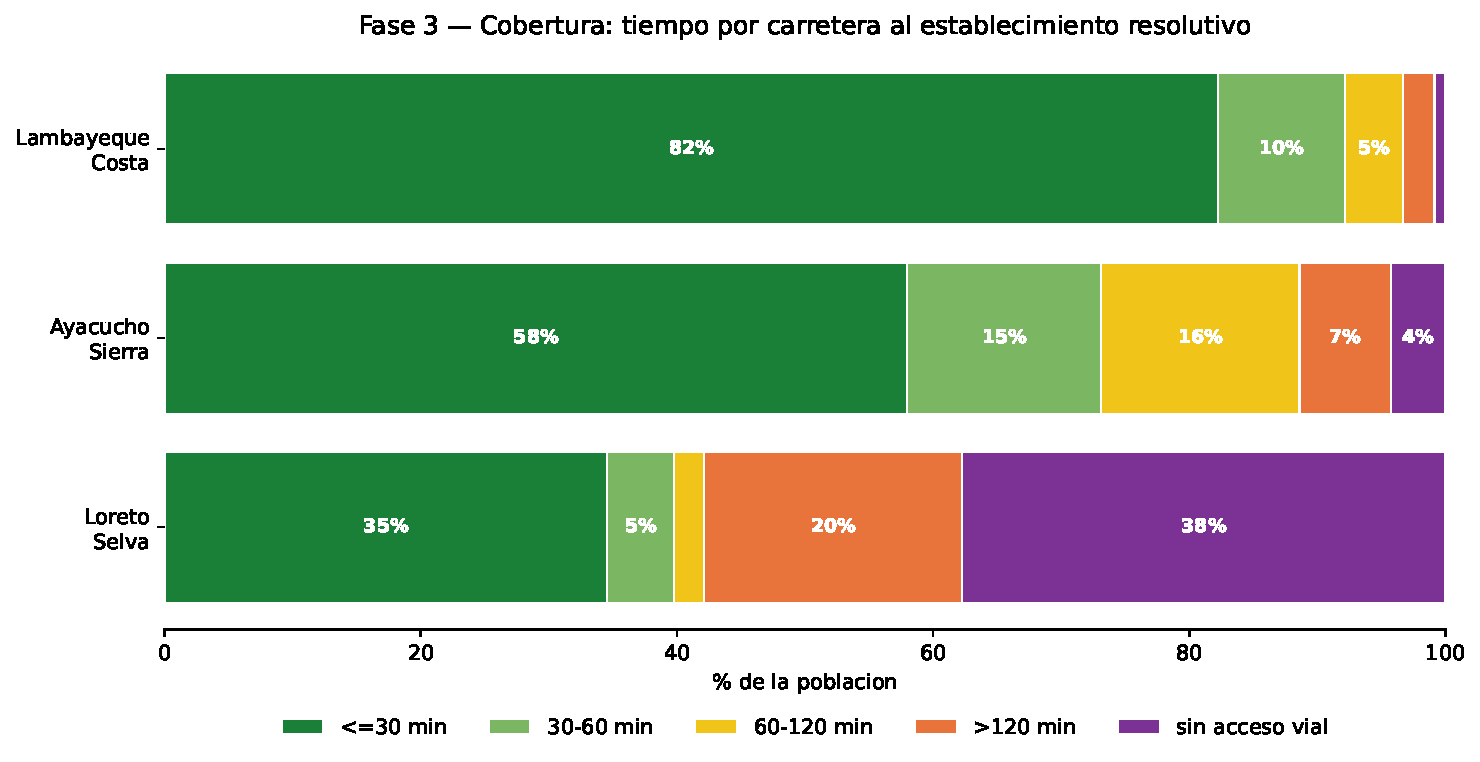
\includegraphics[width=0.95\textwidth]{fase3_bandas.pdf}
\caption{Distribución de la población según el tiempo por carretera al establecimiento
resolutivo más cercano. La banda morada agrupa a quienes la red vial no sirve.}
\label{fig:bandas}
\end{figure}

El \SI{72.2}{\percent} de la población del ámbito alcanza un establecimiento resolutivo en
menos de una hora, y el \SI{12.2}{\percent} no lo alcanza por carretera. El contraste entre
departamentos es de otro orden que la variación interna de cada uno: en Loreto, sumando
quienes tardan más de dos horas y quienes carecen de acceso vial, el \SI{58}{\percent} de la
población está mal servida.

\subsection{Tiempo de acceso y desigualdad}

\begin{table}[htbp]
\caption{Tiempo de acceso ponderado por poblacion, por departamento}
\label{tab:acceso-dep}
\begin{tabular}{lrrrrr}
\toprule
Departamento & Poblacion & Media (min) & Mediana (min) & p90 (min) & Sin acceso vial (\%) \\
\midrule
LORETO & 778389 & 331.9 & 22.5 & 407.8 & 37.7 \\
AYACUCHO & 715240 & 38.8 & 15.0 & 110.6 & 4.3 \\
LAMBAYEQUE & 1238761 & 19.3 & 7.3 & 49.3 & 0.8 \\
\bottomrule
\end{tabular}
\end{table}


\begin{table}[htbp]
\caption{Desigualdad del tiempo de acceso (Gini ponderado por poblacion)}
\label{tab:gini}
\begin{tabular}{lrrr}
\toprule
Ambito & Poblacion & Gini & Media (min) \\
\midrule
AYACUCHO & 684703 & 0.639 & 38.8 \\
LAMBAYEQUE & 1228317 & 0.633 & 19.3 \\
LORETO & 484710 & 0.864 & 331.9 \\
TOTAL & 2397730 & 0.864 & 88.1 \\
\bottomrule
\end{tabular}
\end{table}


Lambayeque y Ayacucho presentan coeficientes de Gini prácticamente idénticos
($0{,}633$ y $0{,}639$) pese a que el tiempo medio de Ayacucho duplica al de Lambayeque. El
dato ilustra qué mide el índice: \textbf{dispersión, no nivel}. La advertencia es relevante
porque el Gini se aplica habitualmente a variables donde más es mejor, y aquí se aplica al
tiempo de viaje, donde más es peor: un Gini de cero significaría que todos tardan lo mismo, no
que todos estén bien atendidos.

\begin{figure}[H]
\centering
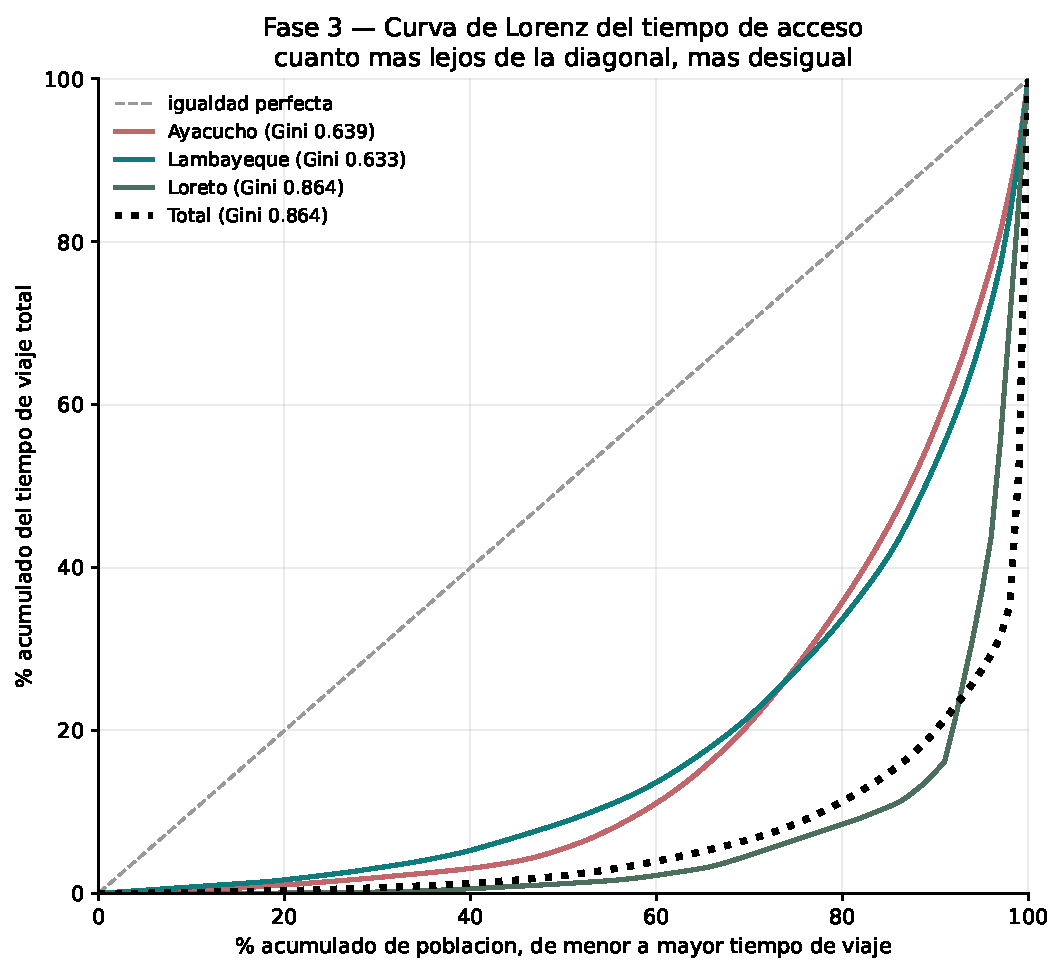
\includegraphics[width=0.62\textwidth]{fase3_lorenz.pdf}
\caption{Curvas de Lorenz del tiempo de acceso. Cuanto más se aleja la curva de la diagonal,
más concentrado está el tiempo total de viaje en una minoría de la población.}
\label{fig:lorenz}
\end{figure}

\subsection{Contraste urbano y rural}

\begin{table}[htbp]
\caption{Acceso urbano frente a rural, ponderado por poblacion}
\label{tab:urbano-rural}
\begin{tabular}{lrrrr}
\toprule
Departamento & Ambito & Poblacion & Media (min) & Sin acceso vial (\%) \\
\midrule
AYACUCHO & rural & 246081 & 55.7 & 9.3 \\
AYACUCHO & urbano & 469158 & 30.7 & 1.6 \\
LAMBAYEQUE & rural & 299620 & 43.0 & 1.5 \\
LAMBAYEQUE & urbano & 939141 & 11.8 & 0.6 \\
LORETO & rural & 200617 & 1394.6 & 72.6 \\
LORETO & urbano & 577771 & 196.1 & 25.6 \\
\bottomrule
\end{tabular}
\end{table}


La brecha entre ámbito urbano y rural es de \num{1.8} veces en Lambayeque y en Ayacucho, y de
\num{7.1} veces en Loreto. La población rural amazónica tarda de media \num{1394} minutos
—unas \num{23} horas— y el \SI{72.6}{\percent} carece de acceso por carretera.

\subsection{Brechas críticas}

\begin{table}[htbp]
\caption{Distritos con peor acceso a capacidad resolutiva. Una raya en la columna de tiempo medio indica que el distrito no tiene ningun punto de demanda con tiempo interpretable: la red vial no lo sirve en absoluto}
\label{tab:brechas}
\begin{tabular}{lrrrrr}
\toprule
\# & Distrito & Departamento & Poblacion & Sin acceso vial (\%) & Media (min) \\
\midrule
1 & OCAÑA & AYACUCHO & 2738 & 100.0 & --- \\
2 & HUACAÑA & AYACUCHO & 715 & 100.0 & --- \\
3 & ANDOAS & LORETO & 8681 & 100.0 & --- \\
4 & BARRANCA & LORETO & 16273 & 100.0 & --- \\
5 & CAHUAPANAS & LORETO & 7859 & 100.0 & --- \\
6 & MORONA & LORETO & 31076 & 100.0 & --- \\
7 & PASTAZA & LORETO & 8067 & 100.0 & --- \\
8 & PARINARI & LORETO & 6732 & 100.0 & --- \\
9 & URARINAS & LORETO & 16535 & 100.0 & --- \\
10 & LAS AMAZONAS & LORETO & 9128 & 100.0 & --- \\
11 & TORRES CAUSANA & LORETO & 5084 & 100.0 & --- \\
12 & ROSA PANDURO & LORETO & 215 & 100.0 & --- \\
13 & TENIENTE MANUEL CLAVERO & LORETO & 4942 & 100.0 & --- \\
14 & ALTO TAPICHE & LORETO & 1932 & 100.0 & --- \\
15 & EMILIO SAN MARTIN & LORETO & 7193 & 100.0 & --- \\
16 & MAQUIA & LORETO & 7889 & 100.0 & --- \\
17 & YAGUAS & LORETO & 2359 & 97.5 & 4903.7 \\
18 & TENIENTE CESAR LOPEZ ROJAS & LORETO & 6912 & 89.1 & 3.2 \\
19 & YAVARI & LORETO & 14688 & 89.1 & 4919.5 \\
20 & TIGRE & LORETO & 8741 & 86.8 & 80.8 \\
\bottomrule
\end{tabular}
\end{table}


\subsection{Cruce con la pobreza distrital}

\begin{table}[htbp]
\caption{Relacion entre acceso y pobreza distrital (correlacional, no causal)}
\label{tab:pobreza}
\begin{tabular}{lrrrrr}
\toprule
Ambito & Distritos & Pearson $r$ & $p$ (Pearson) & Spearman $\rho$ & $p$ (Spearman) \\
\midrule
AYACUCHO & 104 & 0.229 & 0.019 & 0.252 & 0.010 \\
LAMBAYEQUE & 38 & 0.798 & $<$0.001 & 0.563 & $<$0.001 \\
LORETO & 36 & 0.186 & 0.278 & 0.223 & 0.191 \\
TOTAL & 178 & 0.136 & 0.071 & 0.470 & $<$0.001 \\
\bottomrule
\end{tabular}
\end{table}


\begin{figure}[H]
\centering
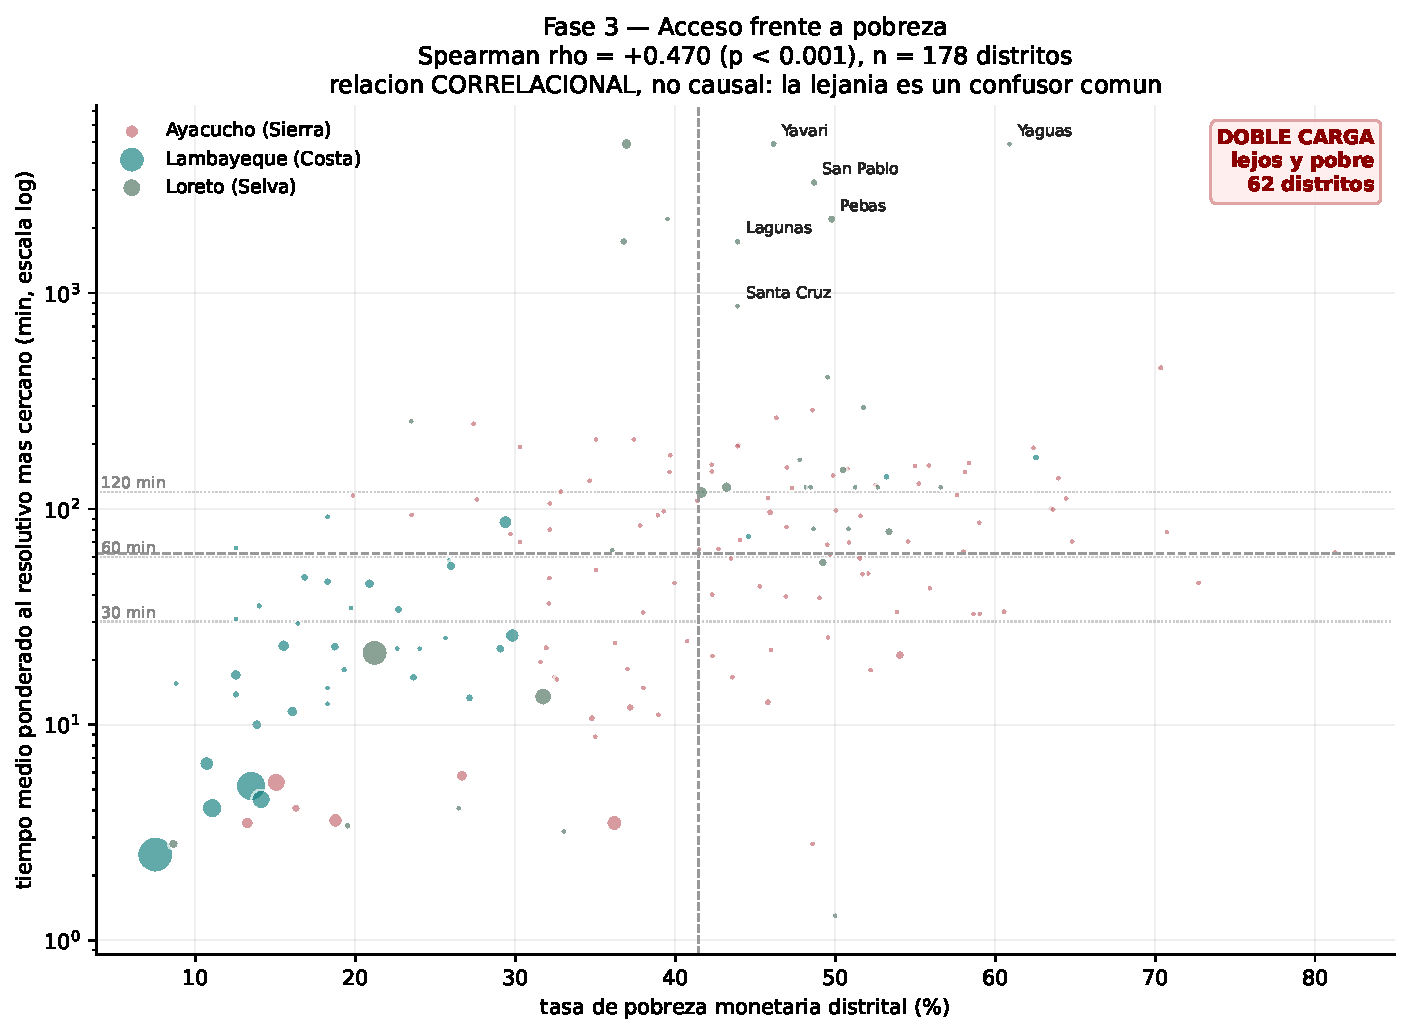
\includegraphics[width=0.78\textwidth]{fase3_pobreza.pdf}
\caption{Acceso frente a pobreza monetaria distrital. Escala logarítmica en el eje vertical:
en escala lineal los distritos amazónicos comprimen al resto contra el eje.}
\label{fig:pobreza}
\end{figure}

La correlación más fuerte se encuentra en el departamento con \emph{mejor} acceso
(Lambayeque, $r = 0{,}798$, $p < 0{,}001$) y desaparece en el peor (Loreto, $p = 0{,}278$). La
lectura es que en la Amazonía la geografía determina la distancia con independencia de la
condición socioeconómica, mientras que en la costa —donde existe red vial en todo el
territorio— la variación residual del acceso sí acompaña a la pobreza.

\textbf{La relación es correlacional, no causal.} Ambas variables comparten un confusor
evidente, la lejanía, que las mueve simultáneamente; tampoco puede descartarse causalidad
inversa. El dato sirve para priorizar, no para explicar. Con ese criterio, \num{62} distritos
quedan simultáneamente por encima de la mediana de pobreza y de tiempo de acceso:
\num{420053} habitantes, el \SI{15.4}{\percent} del ámbito.

% =====================================================================================
\section{Discusión}

\subsection{Red vial frente a línea recta}

El factor de rodeo —kilómetros por carretera divididos entre kilómetros en línea recta—
confirma la hipótesis de partida en dos de los tres departamentos y la rompe en el tercero:
\num{2.14} en Ayacucho, donde las carreteras andinas obligan a recorrer el doble; \num{1.29}
en Lambayeque, de malla plana y densa; y \num{1.06} en Loreto.

Ese último valor es implausible: implicaría que las carreteras amazónicas son casi rectas. La
causa resultó ser el enganche a la red. Midiendo la distancia entre cada centro poblado y la
vía más próxima:

\begin{table}[H]
\centering
\caption{Distancia de enganche a la red vial, en metros.}
\label{tab:snap}
\small
\begin{tabular}{lrrr}
\toprule
\textbf{Departamento} & \textbf{Mediana} & \textbf{p90} & \textbf{Máximo} \\
\midrule
Lambayeque & \num{107} & \num{543} & \num{10178} \\
Ayacucho & \num{207} & \num{2289} & \num{10522} \\
Loreto & \num{8901} & \num{43763} & \num{133754} \\
\bottomrule
\end{tabular}
\end{table}

En la costa y la sierra el centro poblado mediano está a \num{100}--\num{200} metros de una
carretera; en Loreto, a casi \num{9} kilómetros. El factor de \num{1.06} era un artefacto: el
numerador no incluía el tramo omitido. Esta comparación justifica el tratamiento
\texttt{fuera\_de\_red} descrito en la metodología.

\subsection{Robustez del umbral}

La conclusión sobre Loreto no depende del valor elegido para el umbral. Aun con el criterio
más permisivo imaginable —\SI{10}{\kilo\meter}, más de dos horas caminando—, la población
fuera de la red vial cae a \SI{0.0}{\percent} en Ayacucho y \SI{0.1}{\percent} en Lambayeque,
pero se mantiene en \SI{24.0}{\percent} en Loreto. El contraste no se disuelve al relajar el
criterio: se acentúa.

\begin{figure}[H]
\centering
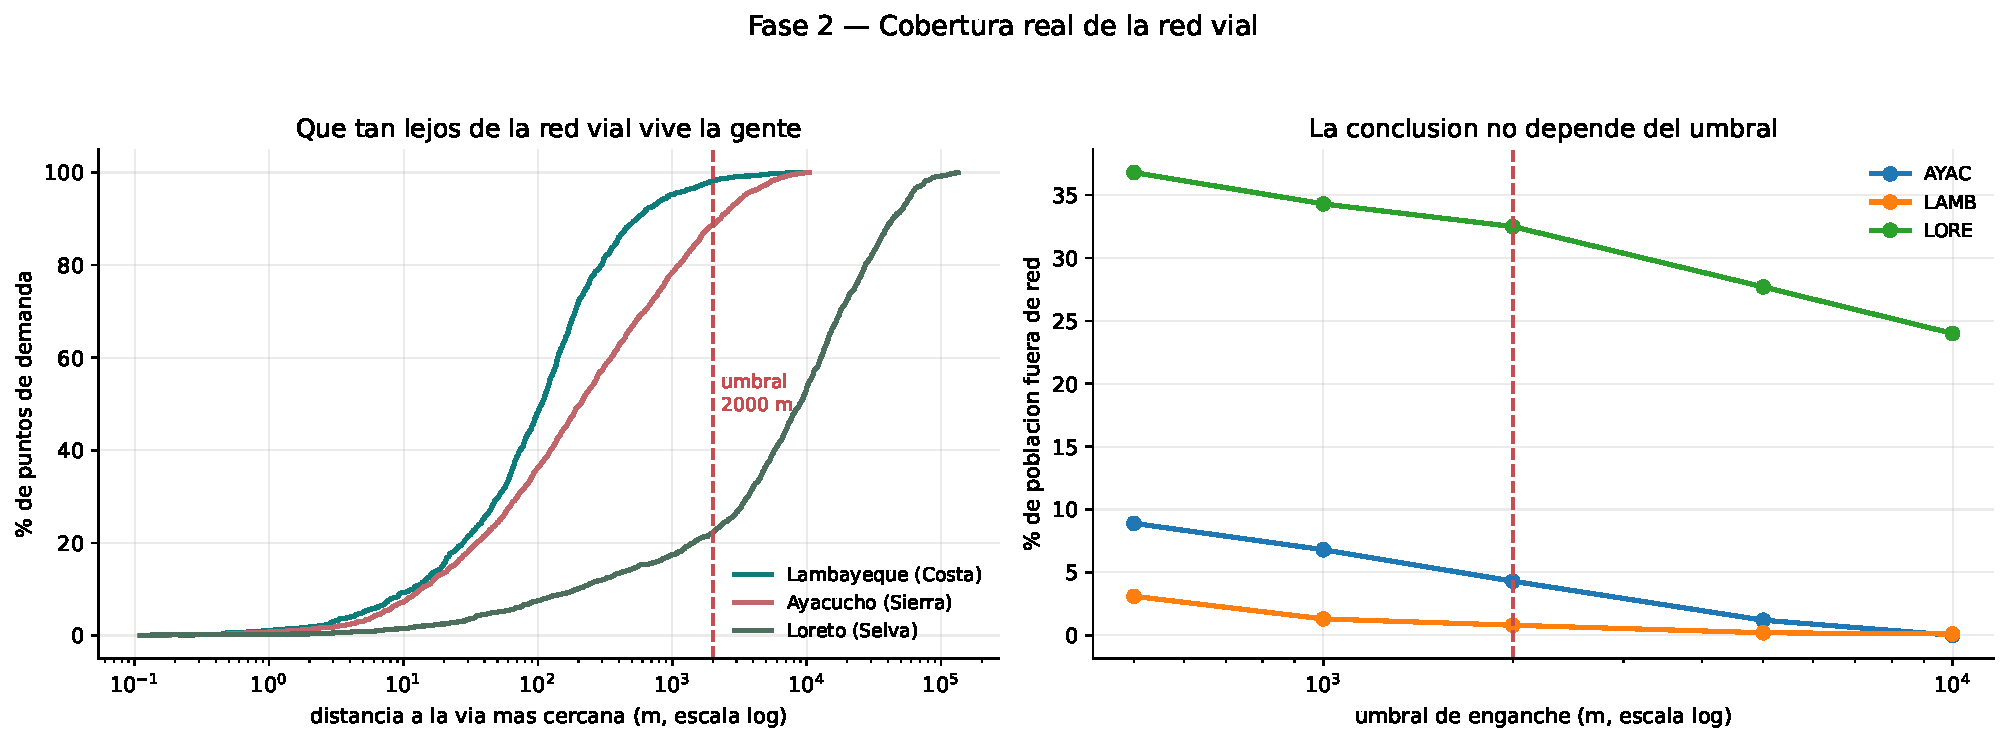
\includegraphics[width=0.95\textwidth]{fase2_snapping.pdf}
\caption{Izquierda: distribución acumulada de la distancia a la vía más próxima.
Derecha: análisis de sensibilidad del umbral de enganche.}
\label{fig:snap}
\end{figure}

\subsection{El modo de transporte cambia la respuesta}

La razón entre el tiempo caminando y en automóvil no es constante: \num{12.6} en Lambayeque,
\num{10.5} en Ayacucho y \num{6.5} en Loreto. La penalización por caminar es \emph{menor} en
la Amazonía porque su red vial es tan escasa que el automóvil tampoco aprovecha gran cosa.

Más relevante para la planificación: \textbf{el establecimiento más cercano cambia según el
modo entre el \SI{17}{\percent} y el \SI{47}{\percent} de los puntos}. Un protocolo de
referencia de emergencias que hable del ``hospital más cercano'' sin especificar el medio de
transporte se equivoca en aproximadamente uno de cada tres casos.

\subsection{Un componente vial aislado}

Al evaluar qué ascenso de un establecimiento I-3 o I-4 a categoría resolutiva ganaría más
cobertura, doce establecimientos distintos —repartidos en ocho distritos de Loreto y sobre un
área de \num{238} por \num{276} kilómetros— resultaron alcanzar \emph{exactamente} los mismos
\num{290} centros poblados, sin una sola diferencia entre los conjuntos. Todos pertenecen al
mismo componente aislado de la red vial amazónica, desconectado del resto del país.

De esos \num{290} puntos, \num{251} (el \SI{87}{\percent}) carecen hoy de acceso resolutivo
por carretera, y representan \num{105856} habitantes. La implicación de política es directa:
dentro de ese componente, la pregunta sobre cuál establecimiento ascender no tiene una
respuesta mejor que otra —cualquiera rinde lo mismo— y la decisión debe tomarse por criterios
de costo, personal o infraestructura existente.

\subsection{El sistema sí funciona de cerca}

El tiempo caminando al establecimiento más cercano \emph{de cualquier categoría} desde los
puntos urbanos es de \num{4.3} minutos en Ayacucho, \num{7.0} en Lambayeque y \num{5.8} en
Loreto. El contraste con el resto del estudio es el hallazgo: para la atención primaria
cotidiana el sistema responde. \textbf{La brecha no está en la atención primaria sino en la
capacidad resolutiva}: cinco minutos hasta una posta que puede estabilizar, frente a
\num{47}--\num{126} minutos hasta un establecimiento que puede operar.

% =====================================================================================
\section{Limitaciones}
\label{sec:limitaciones}

\begin{enumerate}
\item \textbf{Un tercio del registro carece de georreferencia.} \num{13176} de \num{36004}
establecimientos nacionales (\SI{36.6}{\percent}) no tienen coordenadas. La oferta está por
tanto subestimada y los tiempos calculados son, si acaso, pesimistas. Es la limitación de
mayor impacto sobre los resultados.

\item \textbf{WorldPop subestima la población amazónica.} El producto \emph{constrained} solo
asigna población donde detecta edificación desde satélite, y los asentamientos dispersos bajo
dosel arbóreo no se detectan. La población imputada a Loreto (\num{778389}) queda un
\SI{24}{\percent} por debajo de la proyección oficial. Ayacucho y Lambayeque se reproducen con
desviaciones del \SI{7}{\percent} y el \SI{5}{\percent}.

\item \textbf{Conflictos sin resolver entre coordenada y UBIGEO.} \num{1369} establecimientos
declaran un distrito distinto de aquel en el que caen sus coordenadas. No existe información
para decidir cuál de los dos campos es erróneo, de modo que se conservan etiquetados en lugar
de sobrescribir uno con el otro y fabricar una precisión inexistente.

\item \textbf{La población se asigna por proximidad euclidiana}, no por red vial. En valles
encajonados y en la selva, la población más próxima en línea recta no siempre gravita hacia
ese centro poblado.

\item \textbf{El muestreo no captura la varianza intradistrital.} Si un distrito contiene dos
centros poblados con accesos muy distintos y solo uno entra en la muestra, el promedio
distrital hereda su valor. La estratificación garantiza representación de todos los distritos,
no de toda la heterogeneidad interna.

\item \textbf{Sesgo de cobertura rural en OpenStreetMap.} Lo que no está mapeado no existe
para el motor de ruteo, y ese sesgo afecta desproporcionadamente a las zonas que este estudio
busca medir. Parte de lo que se reporta como ausencia de red vial podría ser ausencia de
cartografía.

\item \textbf{El registro rota mes a mes.} Entre los cortes de abril y agosto de 2026 hubo
\num{46} altas, \num{17} cambios de categoría y \num{30} cambios de estado; dos
establecimientos ganaron capacidad resolutiva y uno la perdió. Los resolutivos pasaron de
\num{45} a \num{48} en cuatro meses, casi un \SI{7}{\percent}. \textbf{El resultado tiene fecha
de caducidad}, y la fecha del corte forma parte del resultado.

\item \textbf{Se ignora la capacidad de los establecimientos.} El análisis trata cada
establecimiento resolutivo como infinitamente disponible. No se modela número de camas,
personal ni saturación, de modo que el ``acceso'' medido es geográfico, no efectivo.

\item \textbf{No se dispone de datos de ambulancias ni de traslados fluviales.} En Loreto el
transporte real de emergencias es fluvial o aéreo; este estudio mide exclusivamente la red
vial y por eso su conclusión principal es, precisamente, que esa red no sirve allí.

\item \textbf{La tabla de pobreza carece de procedencia documentada.} No consta su año ni su
fuente exacta, y no cubre cinco distritos de creación reciente. Las variables de PBI per cápita
e IDH de esa misma tabla se descartaron por traer un único valor departamental repetido en
cada distrito, lo que habría producido correlaciones espurias.
\end{enumerate}

% =====================================================================================
\section{Conclusiones y recomendaciones}

\paragraph{Conclusión principal.} El acceso a capacidad resolutiva en el Perú no es
primordialmente un problema de cantidad de establecimientos sino de \textbf{concentración
geográfica}. Los tres departamentos presentan una razón de habitantes por establecimiento
resolutivo muy parecida (\num{55600} a \num{68800}), y sin embargo la población sin acceso
vial va del \SI{0.8}{\percent} al \SI{38}{\percent}. Lo que cambia no es cuántos hay, sino
dónde están.

\begin{figure}[H]
\centering
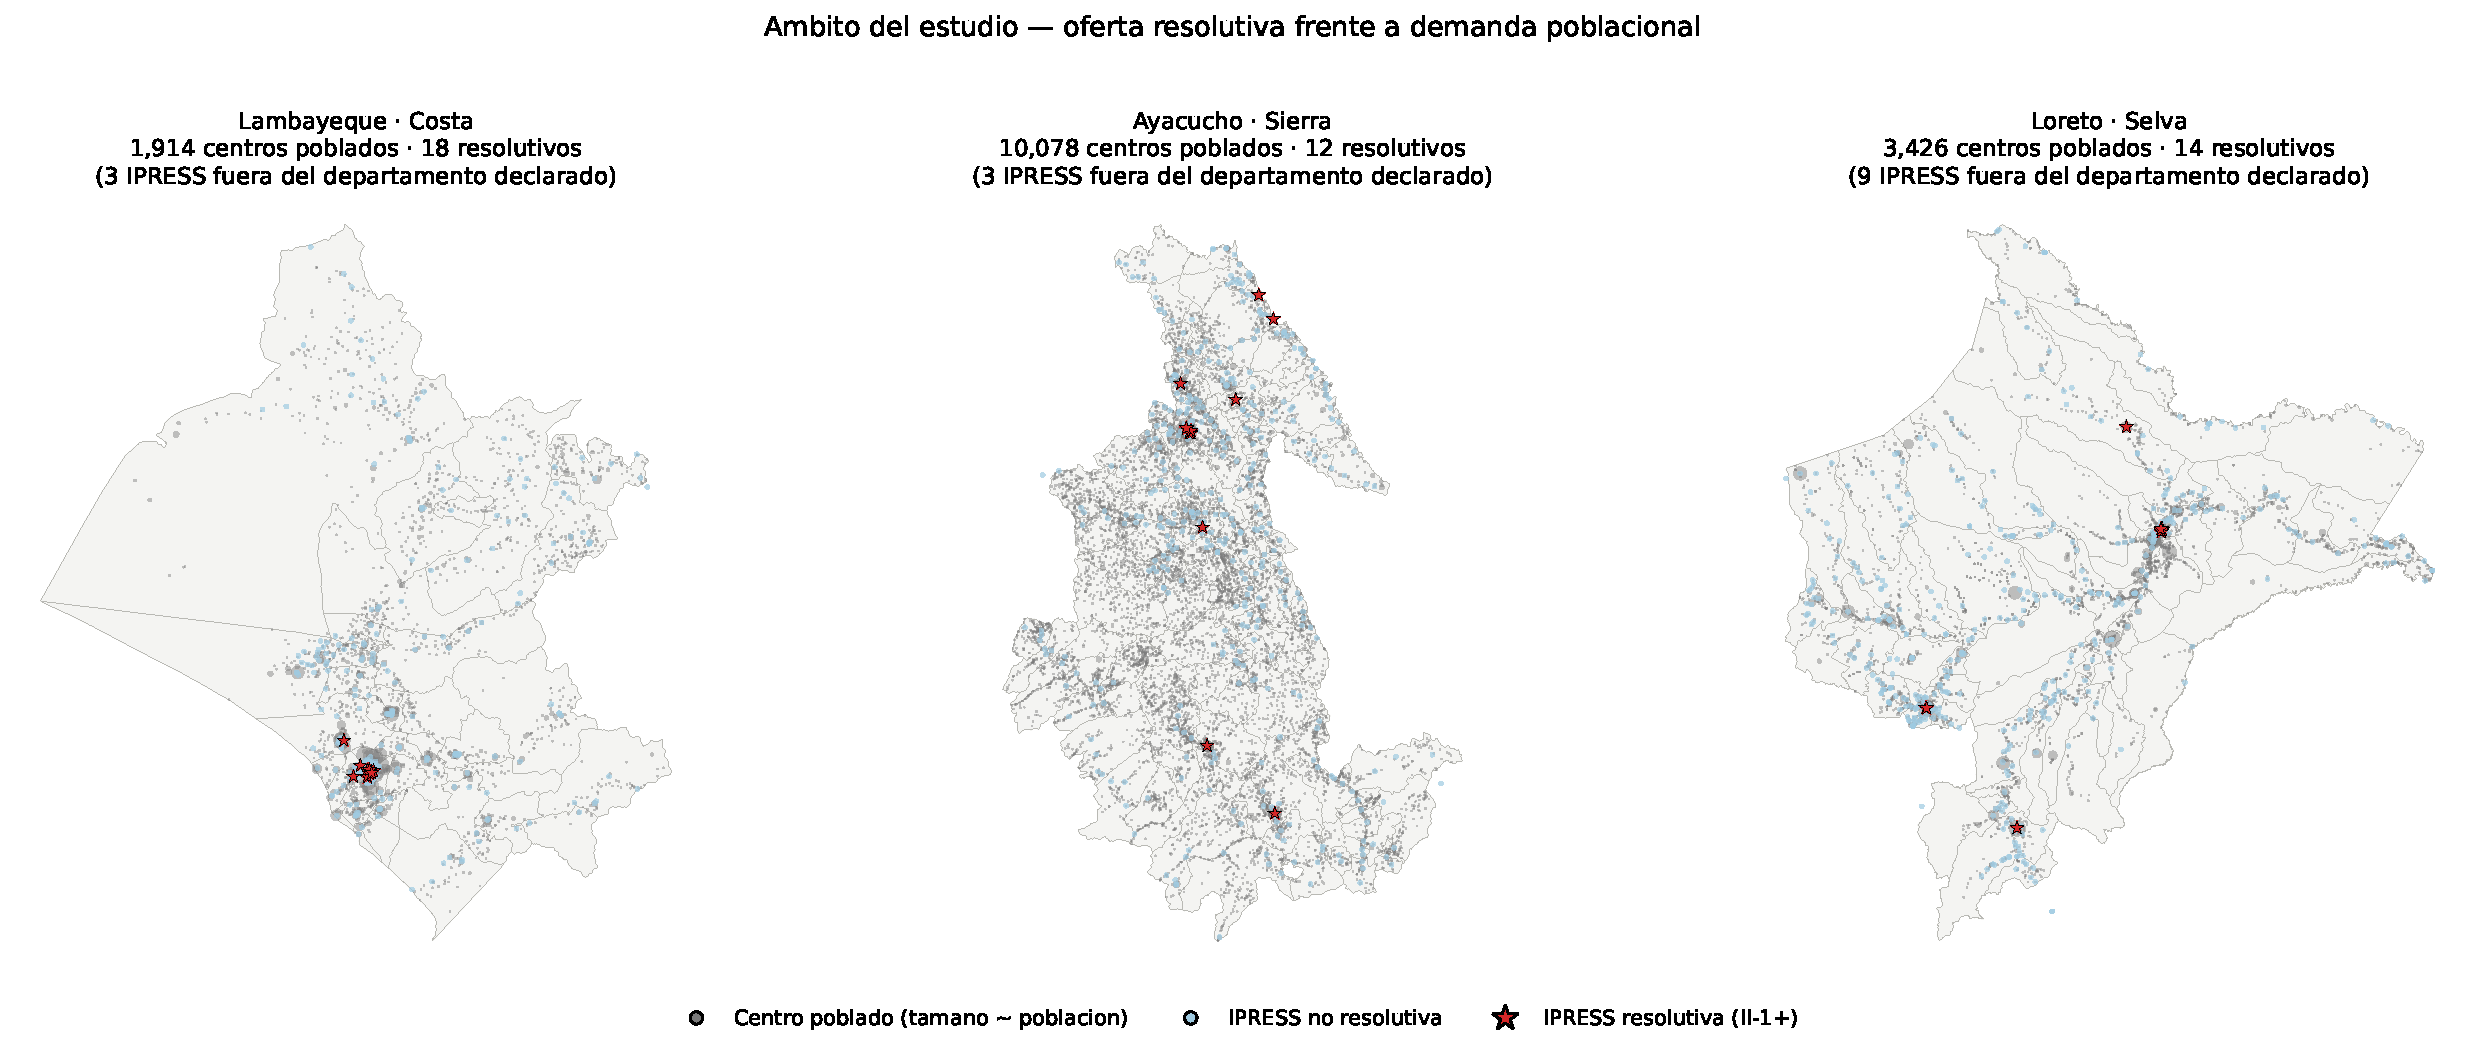
\includegraphics[width=0.95\textwidth]{fase1_ambito.pdf}
\caption{Oferta resolutiva frente a demanda poblacional. En Lambayeque los establecimientos
resolutivos se concentran casi por completo en el núcleo urbano de Chiclayo.}
\label{fig:ambito}
\end{figure}

\paragraph{Recomendaciones.}
\begin{enumerate}
\item \textbf{Georreferenciar el registro antes de planificar.} Un registro nacional de
prestadores con un tercio de las entradas sin coordenadas no permite planificar cobertura
territorial. Antes de decidir dónde ubicar el próximo hospital hay que poder ubicar los que ya
existen.

\item \textbf{No medir el acceso amazónico con una red vial.} Para Loreto se requiere un
modelo de accesibilidad fluvial. Aplicarle el instrumento vial produce cifras optimistas: al
restringir el análisis a los puntos que la carretera sirve, Loreto aparenta un acceso mediano
mejor que el de Ayacucho, cuando lo que ocurre es que la red solo llega allí donde ya hay
hospital.

\item \textbf{Priorizar los \num{62} distritos de doble carga}, más pobres y peor comunicados
que la mediana, donde viven \num{420053} personas.

\item \textbf{Especificar el modo de transporte en los protocolos de referencia}, dado que el
establecimiento más cercano cambia entre el \SI{17}{\percent} y el \SI{47}{\percent} de los
casos según se viaje en automóvil, bicicleta o a pie.

\item \textbf{Tratar la conectividad del componente vial como la variable de decisión} en la
Amazonía. Ascender cualquiera de los doce establecimientos del componente aislado identificado
beneficia a las mismas \num{290} comunidades; ascender los doce no beneficia a ninguna más.
\end{enumerate}

% =====================================================================================
\section*{Reproducibilidad}
\addcontentsline{toc}{section}{Reproducibilidad}

Todas las cifras, tablas y figuras de este documento proceden del pipeline del repositorio.
Ninguna está tecleada a mano: las tablas se incorporan con \verb|\input| desde
\texttt{report/tablas/} y se generan con \texttt{DataFrame.to\_latex} y \texttt{booktabs}; las
figuras se exportan en PDF vectorial desde \texttt{matplotlib}. El documento completo se
regenera con:

\begin{verbatim}
    python run_pipeline.py            # fases 1 a 3, con verificacion automatica
    python run_pipeline.py --phase 5  # recompila este PDF con las cifras vigentes
    streamlit run app.py              # dashboard interactivo
\end{verbatim}

El pipeline aplica \num{179} comprobaciones automáticas sobre sus propias salidas
—consistencia matemática, implicaciones lógicas, coherencia entre archivos y cumplimiento de
los requisitos del enunciado— y se detiene si alguna falla.

% =====================================================================================
\begin{thebibliography}{9}

\bibitem{renipress} SUSALUD (2026). \emph{Registro Nacional de Entidades Prestadoras de
Servicios de Salud (RENIPRESS)}, cortes del 30-04-2026 y 31-08-2026. Plataforma Nacional de
Datos Abiertos.

\bibitem{ign-ccpp} Instituto Geográfico Nacional (2020). \emph{Centros Poblados del Perú},
escala 1:100\,000. Plataforma Nacional de Datos Abiertos.

\bibitem{ign-dist} Instituto Geográfico Nacional. \emph{Límites Distritales del Perú}.
Plataforma Nacional de Datos Abiertos.

\bibitem{worldpop} WorldPop (2020). \emph{Global High Resolution Population Denominators
Project}. University of Southampton. \url{https://dx.doi.org/10.5258/SOTON/WP00660}

\bibitem{osm} OpenStreetMap contributors / Geofabrik GmbH (2026). \emph{Peru OSM extract}.
Open Database License.

\bibitem{osrm} Luxen, D. y Vetter, C. (2011). \emph{Real-time routing with OpenStreetMap
data}. Proceedings of the 19th ACM SIGSPATIAL International Conference on Advances in
Geographic Information Systems, pp. 513--516.

\end{thebibliography}

\end{document}
